	Let's consider the following model:
\begin{equation}
	\left\{
	\begin{aligned}
		\ \Delta c_{t+1} & = \mu + x_t + \varepsilon_{t+1}^c \\
		\ x_t & = \rho x_{t-1} + \varepsilon_{t}^x \\
		\ \Delta d_{t+1} & = \lambda x_t + \varepsilon_{t+1}^d
	\end{aligned}
	\right.
\end{equation}
where $\varepsilon_t^i\iid \mathcal{N}\left(\mu, \sigma_i^2\right)$. The Utility Function is given by 
\begin{equation}
	U_t = \left((1-\delta) C_t^{\alpha} + \delta \ \E_t\left[U_{t+1}^{1-\gamma}\right]^\theta\right)^{\frac{1}{\alpha}},
\end{equation}
where 
\begin{equation}
	\alpha = 1 - \frac{1}{\psi}, \quad\quad \theta = \frac{\alpha}{1-\gamma},
\end{equation}
with $\gamma$ and $\psi$ being the risk aversion and intertemporal elasticity of substitution parameters, respectively. The Stochastic Discount Factor is given by 
\begin{equation}
	M_{t+1} = \delta^\zeta \e{-\Delta c_{t+1}\frac{\zeta}{\psi}} \e{(\zeta-1)r_{c,t+1}},
\end{equation}
where $\zeta =1/\theta$ (and it's the $\theta$ in Bansal and Yaron (2004)), and
\begin{equation}
	R_{c,t+1} = \frac{P_{t+1}+C_{t+1}}{P_t},
\end{equation}
i.e., if we set $m_{t+1} = \log M_{t+1}$, then
\begin{equation}\label{mt}
	m_{t+1} = \zeta \log\delta - \frac{\zeta}{\psi}\Delta c_{t+1} + (\zeta-1)r_{c,t+1}.
\end{equation}
Under No Arbitrage,
\begin{equation}\label{na}
	1 = \E_t\left[\e{m_{t+1} + r_{c,t+1}}\right].
\end{equation}
Note that
$$
m_{t+1} + r_{c,t+1} = \zeta \log\delta - \frac{\zeta}{\psi}\Delta c_{t+1} + \zeta r_{c,t+1}.
$$
On the other hand,
$$
\begin{aligned}
	r_{c,t+1} &= \log \frac{P_{t+1}+C_{t+1}}{P_t} = \log \left[\frac{P_{t+1}+C_{t+1}}{C_{t+1}}\frac{C_{t+1}}{C_t}\frac{C_t}{P_t}\right] \\
	&= \log\left[\frac{P_{t+1}+C_{t+1}}{C_{t+1}}\right] + \log\frac{C_{t+1}}{C_t} + \log \frac{C_t}{P_t} = \log\left[1+ \e{pc_{t+1}}\right] + \Delta c_{t+1} - pc_{t}.\\		
\end{aligned}
$$
Now note that if we define $f(x) = \log (1+g(x))$, where $g(x) = \e{x}$, its first-order Taylor polynomial around $\pcbar = \E[pc_t]$ is given by
$$
		h(pc_{t+1}) = \log(1 + g(\pcbar)) + \frac{g'(\pcbar)}{1+g(\pcbar)} \left(pc_{t+1}-\pcbar\right) = \kappa_{0,c} + \kappa_{1,c} pc_{t+1},
$$
where 
\begin{equation}\label{eq:kappas_c}
	\kappa_{1,c} = \frac{\e{\pcbar}}{1+\e{\pcbar}}, \quad\quad \kappa_{0,c} = \log\left(1+\e{\pcbar}\right)  -\kappa_{1,c}\pcbar.
\end{equation}
Therefore, if we conjecture that $pc_t = \pcbar + b_c x_t$, then
$$
	\begin{aligned}
		m_{t+1} + r_{c,t+1} &= \zeta \log\delta - \frac{\zeta}{\psi}\Delta c_{t+1} + \zeta\left(\kappa_{0,c} + \kappa_{1,c} pc_{t+1} + \Delta c_{t+1} - pc_{t}\right)\\
		&= \zeta\left([\log \delta + \kappa_{0,c}] +\left[1-\frac{1}{\psi}\right] \Delta c_{t+1} + \kappa_{1,c}pc_{t+1}-pc_t\right)\\
		&=\zeta\left([\log \delta + \kappa_{0,c} + \pcbar(\kappa_{1,c}-1)] +\alpha \Delta c_{t+1} + b_c(\kappa_{1,c}x_{t+1}-x_t)\right)\\
		&=\zeta\left([\log \delta + \kappa_{0,c} + \pcbar(\kappa_{1,c}-1)] +\alpha[\mu + x_{t} + \varepsilon_{t+1}^c] + b_c[\kappa_{1,c}(\rho x_t + \varepsilon_{t+1}^x)-x_t]\right)\\
		&=\zeta\left([\log \delta + \kappa_{0,c} + \pcbar(\kappa_{1,c}-1) + \alpha\mu] +\alpha[ x_{t} + \varepsilon_{t+1}^c] + b_c[(\kappa_{1,c}\rho -1)x_t + \kappa_{1,c}\varepsilon_{t+1}^x]\right)\\
		&= \zeta\left([\log \delta + \kappa_{0,c} + \pcbar(\kappa_{1,c}-1) + \alpha\mu] +[\alpha+b_c(\kappa_{1,c}\rho-1)]x_t + \alpha \varepsilon_{t+1}^c  + \kappa_{1,c}b_c\varepsilon_{t+1}^x)\right)\\
		&= \zeta\left(\tau  +[\alpha+b_c(\kappa_{1,c}\rho-1)]x_t + \alpha \varepsilon_{t+1}^c  + \kappa_{1,c}b_c\varepsilon_{t+1}^x)\right).
	\end{aligned}
$$
with 
\begin{equation}
	\tau = \log \delta + \kappa_{0,c} + \pcbar(\kappa_{1,c}-1) + \alpha
\end{equation}
Therefore,
$$
	\begin{aligned}
		1 &= \E_{t-1}\left[\e{m_{t+1}+r_{c,t+1}}\right]\\
		&= \e{{\zeta} \tau }\e{\zeta[\alpha+b_c(\kappa_{1,c}\rho-1)]x_t }\E_t\left[\e{\zeta\left( \alpha \varepsilon_{t+1}^c  + \kappa_{1,c}b_c\varepsilon_{t+1}^x)\right)}\right].
	\end{aligned} 
$$
Therefore, since $x_t$ is still random, and $( 1, x_t)$ is an orthogonal basis in $\mathcal{L}^2$, then we need for that equality to be true that
$$
\alpha+b_c(\kappa_{1,c}\rho-1) = 0,
$$
which is equivalent to
\begin{equation}\label{eq:bc}
	b_c = \frac{\alpha}{1-\kappa_{1,c}\rho}.
\end{equation}
Therefore,
\begin{equation}
	pc_{t} = \pcbar +  \frac{\alpha}{1-\kappa_{1,c}\rho}x_t.
\end{equation}
Hence,
\begin{equation}
	\begin{aligned}
		r_{c,t+1} &= \kappa_{0,c} + \kappa_{1,c}\left[\pcbar + b_c x_{t+1}\right] - \pcbar - b_c x_t + \mu + x_t + \varepsilon_{t+1}^c\\
		&= \left[\kappa_{0,c} + (\kappa_{1,c}-1)\pcbar + \mu\right] + \kappa_{1,c} b_c [\rho x_{t} + \varepsilon_{t+1}^x] - b_c x_t + x_t + \varepsilon_{t+1}^c\\
		&= \bar{r} + \left[b_c\left(\kappa_{1,c}\rho-1\right) + 1\right]x_t + \kappa_{1,c} b_c \varepsilon_{t+1}^x + \varepsilon_{t+1}^c\\
		&= \bar{r} + \left[1-\alpha\right]x_t + \kappa_{1,c} b_c \varepsilon_{t+1}^x + \varepsilon_{t+1}^c\\
		&= \bar{r} + \frac{1}{\psi}x_t +  \frac{\alpha\kappa_{1,c}}{1-\kappa_{1,c}\rho} \varepsilon_{t+1}^x + \varepsilon_{t+1}^c,\\
	\end{aligned}
\end{equation}
with
\begin{equation}
	\bar{r} = \kappa_{0,c} + (\kappa_{1,c}-1)\pcbar + \mu = \log\left(1+\e{\pcbar}\right) - \pcbar + \mu.
\end{equation}
Note that
$$
\log\left(1+\e{\pcbar}\right) - \pcbar = \log\left(\frac{1+\widebar{PC}}{\widebar{PC}}\right) = \log\left(1+\e{-\pcbar}\right)\approx 0
$$
as long as $\pcbar$ is sufficiently high. Hence, just by looking at Figure \ref{fig:fig1}, we can conclude that it is reasonable to assume that
$$
	\bar{r} = \mu + \log\left(1+\e{-\pcbar}\right)\approx \mu.
$$
Hence,
\begin{equation}
	r_{c,t+1} = \mu + \frac{1}{\psi}x_t +  \frac{\alpha\kappa_{1,c}}{1-\kappa_{1,c}\rho} \varepsilon_{t+1}^x + \varepsilon_{t+1}^c,
\end{equation}
so that $\E[r_{c,t}] = \mu$.
\begin{figure}
	\centering
	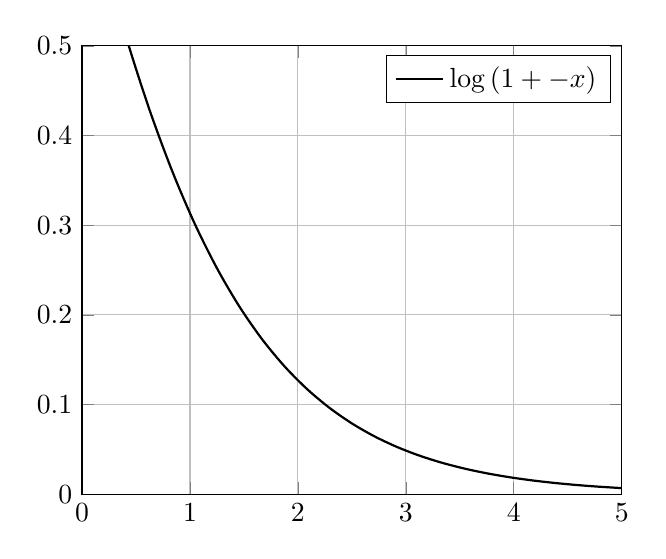
\begin{tikzpicture}
	\begin{axis}[
		grid = both,
		xmin = 0, xmax = 5,
		ymin = 0, ymax = 0.5]
		\addplot[
			domain = 0:5,
			thick,
			smooth,
		] {ln(1+exp(-x))};
		\legend{
			$\log\left(1+\e{-x}\right)$
		}
		
	\end{axis}
\end{tikzpicture}
\caption{$f(x) = \log\left(1+\text{e}^{-x}\right)$ }\label{fig:fig1}
\end{figure}
Now, let's compute the stochastic discount factor:
$$
	\begin{aligned}
		m_{t+1} &= \zeta \log \delta - \frac{\zeta}{\psi} \Delta c_{t+1}+ (\zeta-1) r_{c,t+1}\\
		&= \zeta \log \delta -  \frac{\zeta}{\psi}\left(\mu + x_{t} 
		+ \varepsilon_{t+1}^c\right) + \zeta \left(\mu + \frac{1}{\psi}x_t + b_c \kappa_{1,c} \varepsilon_{t+1}^x + \varepsilon_{t+1}^c\right) - r_{c,t+1}\\
		&= \zeta\left[\log\delta + \alpha\mu\right] + \zeta b_c \kappa_{1,c} \varepsilon_{t+1}^x + \alpha\zeta \varepsilon_{t+1}^c- r_{c,t+1}\\
		&= \left[\zeta \log \delta + (1-\gamma)\mu \right] +  b_c \kappa_{1,c}\zeta\varepsilon_{t+1}^x + (1-\gamma)\varepsilon_{t+1}^c- r_{c,t+1}\\
		&= \left[\zeta\log\delta + (1-\gamma)\mu - \mu\right] -\frac{1}{\psi}x_t + b_c \kappa_{1,c}(\zeta-1)\varepsilon_{t+1}^x - \gamma\varepsilon_{t+1}^c\\
		&= \left[\zeta\log \delta - \gamma\mu\right] - \frac{1}{\psi}x_t + \frac{\frac{1}{\psi}-\gamma}{1-\rho\kappa_{1,c}}\kappa_{1,c}\varepsilon_{t+1}^x - \gamma\varepsilon_{t+1}^c,
	\end{aligned}
$$
because $\zeta \alpha = 1-\gamma$. Hence, the intercept of the stochastic discount factor is
\begin{equation}\label{eq:mbar}
	\bar{m} = \zeta\log\delta-\gamma\mu.
\end{equation}
Finally, our stochastic discount factor is given by
\begin{equation}\label{eq:sdf}
	m_{t+1} = \bar{m} - \frac{1}{\psi}x_t + \frac{\frac{1}{\psi}-\gamma}{1-\rho\kappa_{1,c}}\kappa_{1,c}\varepsilon_{t+1}^x - \gamma\varepsilon_{t+1}^c.
\end{equation}